\documentclass[11pt]{article}

\usepackage[margin=1in]{geometry}
\usepackage{microtype}
\usepackage{amsmath}
\usepackage{graphicx}
\usepackage{booktabs}
\usepackage{array}
\usepackage[hidelinks]{hyperref}

\graphicspath{{figures/}}

\newcommand{\natex}{\texttt{natex}}
\newcommand{\code}[1]{\texttt{#1}}

\title{\natex{} 0.3.0: Methods for Automated Natural-Experiment Discovery and
Calibrated Inference in Tabular Data}
\author{Hauke Hillebrandt\thanks{University College London. Email:
\texttt{ucjthhi@ucl.ac.uk}. This paper and the underlying \natex{} software were
prepared with substantial assistance from Anthropic's Claude models; the author
reviewed the analyses and text and is responsible for all remaining errors.
Latest version: \url{https://haukehillebrandt.github.io/natex/}.}}
\date{October 2026 \\ \small methods of record for \natex{} v0.3.0, 2026-10-05}

\begin{document}

\maketitle

\begin{abstract}
\noindent \natex{} is an open-source toolkit that searches tabular data for natural
experiments and estimates their effects. This paper is the methods record for the paper
collection built with it. One command runs seven design families: local
regression-discontinuity discovery (LoRD3), subset difference-in-differences discovery
(SuDDDS), known-cutoff regression kink and difference-in-kinks designs, Lasso instrument
search with Anderson--Rubin inference, synthetic-control donor selection, bunching at
declared thresholds, and debiased effect estimation. Discovery never reads the outcome.
Version 0.3.0 enumerates the full role space of treatments, running variables and panels.
It no longer scans only the configurations a heuristic or a language model proposed.
Discovered designs are calibrated by fitted-null Monte Carlo with an honest
discovery/estimation split. Calendar-time kinks are gated on a placebo-calibrated $p$
over at least 19 shifted cutoffs. Designs that cannot be validly tested receive an
\emph{inconclusive} verdict rather than a null. On six public benchmark datasets the
pipeline recovers every published design blind. On eight AI time series the nominal 5\% kink test rejected at 7\% to 88\% of placebo
dates. That is why the nominal $p$ no longer decides any verdict.
\end{abstract}

\section{Introduction}\label{sec:intro}

Natural experiments in observational data are usually found by hand. A researcher knows
a rule, locates its cutoff and checks whether the design holds. Herlands et al.
\cite{herlands2018} proposed to automate the search. Fit a smooth model of treatment
assignment, scan local neighbourhoods for a boundary where assignment jumps, and validate
each boundary. \natex{} \cite{natex} implements that programme together with the subset
scan for difference-in-differences from Herlands's thesis \cite{herlands2020} and the
debiasing layer of Jakubowski et al. \cite{jakubowski2023}. It adds known-cutoff
regression kink and difference-in-kinks designs \cite{card2015,bockerman2025}, Lasso
instrument search \cite{belloni2012}, synthetic-control donor selection
\cite{abadie2010} and bunching tests at declared thresholds \cite{kleven2016}. It is a
Python package with a command-line interface and a Python API.

This paper records the methods as they stand in version 0.3.0. It states each estimand,
the inference of record, and the checks behind every verdict. It then gives two kinds of
evidence. Six backtests show what the procedures recover when the answer is published.
Eight AI time series show how often the nominal kink test rejects at dates where nothing
happened. Two worked examples from October 2026 illustrate the full pipeline on fresh
data. The empirical papers in the collection take their inference rules from here.

Three changes in 0.3.0 matter for reading the collection. First, the scan enumerates
every treatment, running-variable and panel combination that the data profile admits.
An analyst pass, heuristic or language model, orders the scan but no longer bounds it.
Second, a design the pipeline could not validly test is reported as inconclusive. Under
0.2.0 a refused placebo test, an unscannable configuration and a degenerate fit were all
reported as null. Third, a kink in calendar time is judged by its rank among shifted
placebo cutoffs, not by its heteroskedasticity-robust $p$-value. Section~\ref{sec:field}
shows why.

Section~\ref{sec:pipeline} gives the pipeline and the design families.
Section~\ref{sec:discovery} states the discovery statistics. Section~\ref{sec:inference}
states the inference of record. Section~\ref{sec:audit} lists the corrections to the
source papers that the implementation carries. Section~\ref{sec:verdicts} defines the
verdict vocabulary. Section~\ref{sec:evidence} reports the evidence.
Section~\ref{sec:limits} states what the methods cannot do.

\section{Pipeline and design families}\label{sec:pipeline}

A run starts from a CSV file. The intake profiler classifies every column as numeric, binary, categorical or time-like.
It lists panel candidates: unit and time column pairs whose grid covers at least 95\% of
rows. Elapsed-time names such as
\code{days}, \code{days\_since\_x}, \code{week}, \code{period}, \code{wave} and \code{t}
count as time-like. An optional analyst pass proposes column roles, a declarative
preparation plan and a ranked search plan. The default analyst is a deterministic
heuristic that needs no network. Language-model backends are available but advisory:
the same data and seed give bitwise-identical statistics with and without guidance.

The survey command then runs the seven families of Table~\ref{tab:families} in a fixed
order and writes one report with a verdict per family. Each family runs in isolation. An
exception is recorded verbatim and the survey continues. A single
\code{numpy.random.Generator} is spawned once into seven streams in registry order, so a
skipped family never shifts another family's random draws. Same seed, same report.

\begin{table}[t]
\centering
\small
\caption{Design families. ``Discovered'' means the cutoff, subset or instrument set is
searched for; ``declared'' means the user supplies it.}
\label{tab:families}
\begin{tabular}{@{}p{1.5cm}p{3.6cm}p{1.7cm}p{3.9cm}p{4.0cm}@{}}
\toprule
Family & Inputs & Cutoff & Statistic & Output \\
\midrule
rdd & treatment, numeric forcing columns & discovered & LoRD3 max LLR over local hyperplane splits & local effect at the boundary, frozen-side 2SLS \\
did & unit $\times$ time panel, treatment variable & discovered & SuDDDS LLR over covariate subsets and intervention times & DD, synthetic-control or GESS gap with placebo $p$ \\
kink & outcome, running variable, cutoff, bandwidth & declared & right-minus-left local-linear slope change & RKD or DiK marginal response; descriptive slope change in calendar time \\
iv & treatment, instrument pool, controls & discovered & plug-in Lasso first stage, HC1 $F$, Hansen $J$ & 2SLS with Anderson--Rubin set on the estimation half \\
sc & unit $\times$ time outcomes, treated unit, $t_0$ & declared & pre-period fit, post/pre RMSPE ratio & post-period ATT with in-space placebo $p$ \\
bunching & running variable, thresholds & declared & binned-Poisson intercept jump & density jump at the threshold \\
dee & covariates, treatment, outcome, observational CATE estimator & discovered via rdd & GP bias surface, stacked mixture & debiased CATE surface \\
\bottomrule
\end{tabular}
\end{table}

The house rules apply to every family. Discovery never reads the outcome. A failed
computation returns a missing value, never zero. Every stochastic step draws from the one
generator. Where a source paper and its released code disagree with the derivation, the
reconciled audit of Section~\ref{sec:audit} governs.

\section{Discovery statistics}\label{sec:discovery}

\subsection{LoRD3: local regression-discontinuity discovery}\label{sec:lord3}

Let $x_i$ be the forcing columns, $T_i$ the treatment and $y_i$ the outcome. LoRD3 fits
one smooth background model $T_i = f(x_i) + \varepsilon_i$, with $f$ a polynomial of
degree $d$ in the standardised forcing columns. The residual model is heteroskedastic
Normal for a real-valued treatment and Bernoulli with a log-odds offset for a binary
one. The fit reads only $(x, T)$.

The scan visits every data point. The neighbourhood of point $i$ is its $k$ nearest
neighbours in standardised forcing space. Each of the $k-1$ hyperplanes through the
centre and one other neighbour bisects the neighbourhood. A bisection is scored by the
log-likelihood ratio of a two-group shift alternative against a single-shift null. For the Normal model the score is the generalised likelihood ratio of two side means
against one common mean. The weights are $1/\sigma_j^2$ for residual variances
$\sigma_j^2$.
For the Bernoulli model the side offsets are fitted by bracketed Newton steps in
$\log\beta$ with a Firth fallback under separation. A pure-group split, where one side
is all treated, is scored at the boundary likelihood supremum rather than dropped.
Discoveries are ranked by maximum LLR. The responsible forcing columns are read from the
normalised hyperplane normal. The centre lies on every candidate hyperplane, so
membership is explicit: signed distance at least zero is group one.

Defaults are $k=50$, degree $d=1$ and $q=99$ null replicas. For large $n$ a coarse-to-fine
scan scores a seeded subsample of 2{,}000 centres and rescans the top candidates at full
resolution. The share of centres scanned is always reported. On the 44{,}362-row
academic-probation file the coarse-to-fine scan takes about five seconds.

\subsection{The role space}\label{sec:rolespace}

A configuration is a treatment column, a set of forcing columns and, for did, a unit and
time pair. Version 0.3.0 enumerates every profiled binary treatment candidate crossed with every
single non-time-like forcing column. It adds the joint all-forcing candidate per treatment
and every treatment crossed with every profiled panel. Three kinds of column are excluded,
each with its reason recorded. They are time-like forcing columns, columns declared as
outcomes in the preparation plan, and treatments that are a global deterministic step in a
time column. The last case is a mechanical rediscovery of the design's own adoption
boundary and is reported as inconclusive whatever its scan $p$.

A search plan's guessed outcome is not reserved. It stays in the forcing space and is
estimated as an outcome wherever it is not a role. Under 0.2.0 the heuristic reserved the
first numeric column, which on a test fixture removed the planted running variable from
every scan. Every scanned boundary is now estimated against every candidate outcome,
and the report carries a per-outcome table. The scan still never reads any of them.
Configurations are ranked by fitted-null $p$ before raw LLR, because LLRs are not
comparable across forcing dimensions. The report lists what was enumerated, what was
excluded, and what the budget left unscanned.

\subsection{SuDDDS: subset difference-in-differences discovery}\label{sec:suddds}

Panel records $(x_i, t_i, \theta_i, y_i)$ carry categorical covariates $x$, time $t$,
a treatment variable $\theta$ and an outcome $y$. The background model gives every unit
its own effect plus a polynomial in standardised time, solved by least squares. The
residuals $r_i = \theta_i - \hat f(\text{unit}_i, t_i)$ have profile-level variances
$\sigma_i^2$ shrunk towards the global variance with a data-scaled floor. The scan looks for a subset $s$ and a time $T_0$ at which $\theta$ jumps inside a window
$[T_0 - W, T_0 + W)$. A subset is a conjunction over dimensions of unions over values. With
$c_i = r_i/\sigma_i^2$, $b_i = 1/\sigma_i^2$ and $C_1, B_1$ the post-side sums and
$C_2, B_2$ the pre-side sums over $s$, the double-beta score is
\begin{equation}
\mathrm{LLR}(s, T_0) = \frac{C_1^2}{2B_1} + \frac{C_2^2}{2B_2}
  - \frac{(C_1 + C_2)^2}{2(B_1 + B_2)}.
\end{equation}
The corrected single-$\Delta$ statistic profiles the per-profile means out under both
hypotheses and restricts to the window. For a binary $\theta$ the window contrast is
scored with exact Bernoulli log-odds offsets; the Normal model remains available for
parity with the thesis. A global incumbent is kept across all windows and restarts.
A cutoff qualifies only with at least three in-window records on each side. Dimensions
with at most 12 values are enumerated exactly, $2^{k}-1$ subsets per dimension. Default
windows are one eighth, one quarter and one half of the time span, with eight restarts.

\subsection{Known-cutoff kinks}\label{sec:kinks}

The kink estimator fits a separate local polynomial on each side within $|x| \le h$ of a
declared cutoff. Triangular kernel weights and degree one are the defaults. A
kink is always right minus left: $\kappa[Z] = m[Z,\text{right}] - m[Z,\text{left}]$,
with $m$ the one-sided derivative of $E[Z \mid x]$ at zero. Table~\ref{tab:kinks} gives
the estimands. A group difference-in-kinks contrasts a treated group's kink against a
control group's at the same cutoff. It is numerically the stacked DiK estimator with the group indicator in place of the
period indicator. What changes is the identifying assumption, which becomes parallel non-
policy kinks across groups.

\begin{table}[t]
\centering
\small
\caption{Kink estimands. $\kappa[\cdot]$ is the right-minus-left slope change of the
named variable; ``policy'' is the observed policy variable in fuzzy designs.}
\label{tab:kinks}
\begin{tabular}{@{}ll@{}}
\toprule
Design & Estimand \\
\midrule
Sharp RKD & $\kappa[Y] / \text{known policy kink}$ \\
Fuzzy RKD & $\kappa[Y] / \kappa[\text{policy}]$ \\
Sharp DiK & $(\kappa[Y,\text{post}] - \kappa[Y,\text{pre}]) / \text{known policy kink change}$ \\
Fuzzy DiK & $(\kappa[Y,\text{post}] - \kappa[Y,\text{pre}]) / (\kappa[\text{policy},\text{post}] - \kappa[\text{policy},\text{pre}])$ \\
Group DiK & as DiK with group 1 and group 0 in place of post and pre \\
\bottomrule
\end{tabular}
\end{table}

With a unit policy denominator the estimate is a descriptive slope change in outcome
units per unit of the running variable. That is the form every calendar-time kink in the
collection takes. The bandwidth is required. The survey's default, the median absolute distance to the
cutoff, carries no optimality claim. It is reported with a half, one and double bandwidth
grid.

\subsection{Instruments, donors and bunching}\label{sec:others}

Instrument search follows Belloni et al. \cite{belloni2012}. The treatment and the
candidate pool are residualised on the controls. An iterated plug-in Lasso with
heteroskedasticity-robust loadings selects a support; the penalty is
$\lambda = 2c\sqrt{n}\,\Phi^{-1}(1 - \gamma/2p)$ with $c = 1.1$ and
$\gamma = 0.1/\log\max(n,p)$. Post-Lasso OLS gives the first stage. An empty selection
is reported as empty, with a missing $F$. Selection reads only the treatment, the pool
and the controls.

Donor selection follows Abadie, Diamond and Hainmueller \cite{abadie2010}. Candidates
are units observed at every pre-period time of the treated unit. They are scored on the
pre-period trajectory only, and simplex weights are fitted on a scale-normalised
objective. The post-period gap gives the ATT. No covariate weights are fitted.

Bunching at a declared threshold reuses the density statistic of
Section~\ref{sec:battery}. A binned-Poisson regression of counts on signed distance, with
a bin edge pinned at the threshold, tests the intercept jump. Because the threshold
was declared, no selection correction is needed.

\section{Inference of record}\label{sec:inference}

\subsection{Fitted-null Monte Carlo and the honest split}\label{sec:mc}

The significance of a discovered boundary is a parametric bootstrap against the fitted
null. Each replica redraws $T^\ast$ from the fitted background model and reruns the full
scan. Binary replicas are drawn as Bernoulli$(\hat p)$ directly. The $p$-value is the
add-one rank,
\begin{equation}
p = \frac{1 + \#\{\text{replica max LLR} \ge \text{observed max LLR}\}}{q + 1}.
\end{equation}
This is never called exact. The primary post-selection guarantee is an honest split: a
random half of the rows is used for discovery and the disjoint half for estimation. The
selection event is then a function of the discovery half alone, so estimation-half
$p$-values keep their nominal distributions without correction. The same split
separates instrument selection from 2SLS, $J$ and Anderson--Rubin inference.

\subsection{Falsification battery for discovered designs}\label{sec:battery}

Every discovered boundary passes through three checks. Placebo tests fit side-specific
trends in each remaining covariate and test intercept equality at the cutoff, with Holm
correction across covariates \cite{holm1979}. The printed side-mean contrasts were
dropped because any smooth covariate rejects them under a valid design. A density test regresses binned counts of the signed distance along the frozen discovered
normal on a polynomial with an intercept jump, in the spirit of McCrary
\cite{mccrary2008}. It is a falsification check only, because the search selected the
geometry. First-stage relevance is never inferred from a high LLR. The first-stage jump,
its $t$-statistic, a weak-instrument flag and an Anderson--Rubin set
\cite{anderson1949,fieller1954} accompany every local 2SLS estimate.

SuDDDS discoveries are checked for composition and anticipation. The composition check is
a chi-square test of unit counts before and after $T_0$ inside the window. The
anticipation check tests placebo jumps at $T_0$ minus one to three steps, with Holm
correction. A McCrary test on calendar time is
information-free when record times are design-determined, and is not run.

\subsection{Calendar-time kinks: placebo calibration}\label{sec:placebo}

A kink in calendar time asks whether a trend bent at a dated event. No unit sorts
itself across a date, so density arguments give no protection. Identification reduces to
one untestable assumption: nothing else bent the outcome's expected slope at that date.
Two facts make the nominal $p$ unusable as the gate. Aggregate series are serially
correlated, and side-specific local fits absorb low-frequency noise before the residual
scores see it. Table~\ref{tab:ar1} gives the calibration on AR(1) noise. At nominal 5\% the HC1 test
rejects about half the time. A Newey--West covariance still rejects a third of the time at
every lag between 4 and 20.

\begin{table}[t]
\centering
\small
\caption{Empirical size at nominal 5\% of the kink $t$-test on 64 time points of AR(1)
noise with $\rho = 0.75$ and no kink.}
\label{tab:ar1}
\begin{tabular}{@{}lc@{}}
\toprule
Covariance & Empirical size \\
\midrule
HC1 & 0.48 \\
Newey--West, lags 4 to 20 & 0.34 \\
VAR(1) prewhitening & 0.19 \\
\bottomrule
\end{tabular}
\end{table}

The inference of record is therefore a placebo-calibrated $p$. The same estimator, with
the same bandwidth, kernel and covariance, is run at shifted placebo cutoffs. The grid takes the distinct running values in the central 80\% of the support. It drops
any within a quarter bandwidth of the declared cutoff and thins to at most 49 positions
(Appendix~\ref{app:grid}). With $N$ evaluable placebos and $z = \hat\tau/\widehat{se}$,
\begin{equation}
p_{\mathrm{cal}} = \frac{1 + \#\{|z_{\mathrm{placebo}}| \ge |z|\}}{1 + N}.
\end{equation}
The smallest attainable value is $1/(N+1)$. Fewer than 19 positions cannot reach 0.05,
and the cutoff is reported as inconclusive. A seven-placebo grid has a floor of 0.125, so
``0 of 7 placebos reject'' is the floor of the test, not a 5\% finding. Under 0.2.0
several collection papers made exactly that claim.

The grid yields a second number: the share of placebo cutoffs at which the nominal test
rejects at 5\%. This is the empirical size of the nominal test on that series, at dates
where nothing happened. It is reported beside every verdict as a diagnostic. It is not a
power certificate: rejections elsewhere say nothing about whether a bend at the event
date would have been detected. Power is argued from the minimum detectable kink, about
1.96 standard errors against the slope change the claim implies.

The grid also separates bend existence from date attribution. A significant kink at the
declared date together with significant kinks at shifted dates means the series bends
over an era, not at the event. Two further safeguards apply. Cells with at most $d+2$ points raise a small-cell warning.
Leverage near one shrinks squared residuals and overstates HC1 precision. On a 12-point
series the DiK $z$ had $P(|z| \ge 3.63) = 0.080$ under its own fitted null, against a
nominal $3.6\times10^{-4}$. And every estimate reports the lag-one autocorrelation of per-
date mean residuals. A warning fires at 0.25 when no HAC covariance was requested.

\subsection{Effects after discovery}\label{sec:effects}

A SuDDDS effect is tested with a two-sided studentised placebo statistic $|\tau_p /
se_p|$. The placebo subsets are matched in shape to the discovered one, and the add-one
rank is the $p$-value. Fewer than five usable placebos is a refusal and the family
verdict is inconclusive. A synthetic-control effect is tested in space. Every complete donor is refit as pseudo-
treated under the identical selection rule, with the treated unit removed from every
placebo panel. The statistic is the post/pre RMSPE ratio. The gate for this family is
0.10. The add-one $p$ has granularity $1/(n+1)$, so 0.05 is often unattainable with few
donors. The $p$ itself is always reported. Instrument
estimates carry a closed-form Anderson--Rubin set that is reported as found: interval,
disjoint, unbounded or empty. It is never coerced to a finite interval, and it is bounded
exactly when the homoskedastic first-stage $F$ exceeds the AR critical value.

\section{Corrections to the source papers}\label{sec:audit}

Before implementation, all 142 numbered equations and algorithms of the three source
papers were re-derived by one model family. A second model family re-derived them
independently. Disagreements were settled by rendering the disputed pages at 576~dpi. The reconciled
audit lives in the repository and governs whenever code, documentation and the printed
papers disagree. Table~\ref{tab:audit} lists the corrections with design consequences.
Typographical errors in the printed equations are absorbed silently and listed in the
method cards.

\begin{table}[t]
\centering
\small
\caption{Design-level corrections carried by the implementation.}
\label{tab:audit}
\begin{tabular}{@{}p{6.2cm}p{8.6cm}@{}}
\toprule
As printed & In \natex{} \\
\midrule
Randomization test described as exact & Parametric bootstrap against the fitted null, add-one rank; honest split as the post-selection guarantee \\
Bernoulli null drawn as $1\{\hat p + \hat\sigma Z > U\}$, success probability not $\hat p$ & Replicas drawn as Bernoulli$(\hat p)$ \\
Placebo tests on side means, which reject any smooth covariate & Local intercept-continuity contrasts with side-specific trends, Holm-corrected \\
Group-instrument estimator $W = T - \mu$, inconsistent under the paper's DGP & Frozen side-indicator 2SLS, HC1; the printed form is never implemented \\
One-sided 95th-percentile $\hat\tau$ placebo rule & Two-sided studentised statistic, matched placebo shapes, add-one $p$ \\
Density test on an oblique projection with fixed critical values & Binned-Poisson test on the frozen discovered normal, falsification only \\
Scan LLR taken to imply instrument relevance & First-stage jump, $t$, weak flag and AR set reported with every estimate \\
DEE mixture draws a model label per prediction point & One label per posterior draw; analytic mixture covariance with the between-model term \\
Observational estimator fit on the rows that produced the local effects & Experiment-level cross-fitting; chi-square measurement model on $SE^2$ \\
SuDDDS Algorithm 6 keeps no global best; Algorithm 7 scores empty sides & Global incumbent across windows and restarts; three records per side required \\
Algorithm 8 is deletion-only; Algorithm 9 maximises the control MSE & Relax-and-slice repair with exact enumeration up to 12 values; argmin with $+\infty$ start \\
Single-$\Delta$ statistic treats profile means as known & Means profiled out under both hypotheses; window-restricted; both signs scanned \\
Variance floor of $10^{-6}$, absolute & Data-scaled floor; the released code's reverse-neighbour variance indexing is not reproduced \\
\bottomrule
\end{tabular}
\end{table}

\section{Verdicts}\label{sec:verdicts}

Every family ends in one of six statuses (Table~\ref{tab:status}). The distinction that
matters most is between null and inconclusive. Null means the design was testable and
nothing credible surfaced. Inconclusive means the family ran but the test could not be valid. There are five reasons.
A placebo pool has fewer than five usable members. A configuration could not be scanned. A
treatment is a mechanical rediscovery of a constructed time step. A kink, density or DEE
fit is degenerate. A calendar-time kink has fewer than 19 placebo positions. An
inconclusive verdict is never a negative finding and never appears in an abstract.

\begin{table}[t]
\centering
\small
\caption{Family statuses in the survey report.}
\label{tab:status}
\begin{tabular}{@{}lp{10.8cm}@{}}
\toprule
Status & Meaning \\
\midrule
credible & the family ran and its design-specific gate passed \\
null & the family ran, the design was testable, and no credible design surfaced \\
inconclusive & the family ran but the design could not be validly tested \\
skipped & the family did not run: inapplicable by profile, analyst skip, or a runtime gate \\
needs\_input & a requirement only the user can supply is missing, such as a cutoff or an instrument pool \\
failed & the family raised; the error is recorded verbatim and other families are unaffected \\
\bottomrule
\end{tabular}
\end{table}

The credible gates, with $\alpha = 0.05$, are:
\begin{itemize}
\item rdd: scan $p \le \alpha$, placebo battery passed, density $p > \alpha$.
\item did: scan $p \le \alpha$; composition and anticipation checks passed.
\item kink: minimum Holm-adjusted $p$ across the declared cutoffs at or below $\alpha$.
The per-cutoff $p$ is the nominal HC1 $p$ for a cross-sectional running variable and
the placebo-calibrated $p$ for a time-like one.
\item iv: instruments selected, with a strong first stage on both halves of the honest
split.
\item sc: in-space placebo $p$ at or below 0.10.
\item bunching: minimum Holm-adjusted binned-Poisson $p$ at or below $\alpha$.
\item dee: a fitted surface over a usable ensemble.
\end{itemize}
Applicability is decided by declarative predicates over the profile and the user's
declarations. The data values are never read. An analyst may override the heuristic in
either direction. Every override is recorded with its reason.

\section{Evidence}\label{sec:evidence}

\subsection{Backtests on published designs}\label{sec:backtests}

Six public datasets with a published design are run blind: the pipeline is never told
the cutoff, the treated unit or the timing. Table~\ref{tab:backtests} summarises what it
recovers. The runs are the repository's backtest suite, 32 tests in all, and the Prop~99
case has its own note \cite{prop99note}.

\begin{table}[t]
\centering
\small
\caption{Blind backtests. Row counts are after the documented protocol restrictions.}
\label{tab:backtests}
\begin{tabular}{@{}p{3.3cm}p{1.9cm}p{9.4cm}@{}}
\toprule
Dataset & Design & Recovered \\
\midrule
MDRC RDD practice set, 2{,}767 rows & sharp RDD & pretest cutoff at 215; the known effect of about 10 lies inside the 2SLS interval \\
Academic probation (Lindo, Sanders and Oreopoulos 2010), 44{,}362 rows & fuzzy RDD & distance to the probation cutoff ranked first of four forcing candidates; cutoff at 0; 2SLS sign matches the published +0.233 \\
Emergency-department visits (Anderson, Dobkin and Gross 2012), 161 monthly cells & fuzzy RDD & insurance-loss cutoffs at ages 19 and 23 among the top clusters; density negative control holds \\
Inpatient visits (same source), 73 cells & fuzzy RDD & age-23 cutoff on 73 aggregated cells \\
Bavarian council size (Egger and Koethenbuerger 2010), 42{,}005 rows & multi-cutoff RDD & four of five statutory population thresholds are the only top-50 clusters; the fifth ranks 54th \\
Proposition 99 (Abadie, Diamond and Hainmueller 2010), 39 states $\times$ 31 years & SuDDDS and SC & (California, 1989) recovered exactly by all scan methods; Bernoulli-null $p = 0.010$; donor weight 0.955 on the five published donors; ATT $-19.5$ packs; in-space placebo rank 3 of 39 \\
\bottomrule
\end{tabular}
\end{table}

Two Prop~99 details are findings about the estimators rather than the scan. With the corrected two-sided studentised placebo test, the three effect estimates rank 13,
7 and 9 of 39 placebo states. The thesis's claim that all three are significant at 5\%
does not survive. And the in-space placebo rank of 3 of 39 differs from the published 1 of
39. The published figure discards poorly fitting placebos before ranking. That exclusion
is opt-in here.

\subsection{Size of nominal inference in the field}\label{sec:field}

Figure~\ref{fig:size} and Table~\ref{tab:size} report, for eight AI time series, the
share of shifted placebo cutoffs at which the nominal HC1 test rejected at 5\%. The first four are the flagship paper's series \cite{flagship}. The capex series is from
its companion note \cite{capexnote}. The last three are the October 2026 runs of
Section~\ref{sec:worked}. The nominal test rejected at between 7\% and 88\% of
non-event dates. On no series did it hold its size. The placebo-calibrated $p$ reaches its floor on three series. They are the GPQA-Diamond
score at o1-preview and two series at the Mythos announcement: pooled high and critical
CVE publications, and fresh additions to the CISA Known Exploited Vulnerabilities
catalogue. The series with the largest nominal $z$, the GPU-cluster stock at ChatGPT with
$z = 8.95$, has a calibrated $p$ of 0.62. A smooth super-exponential series bends
everywhere.

\begin{figure}[t]
\centering
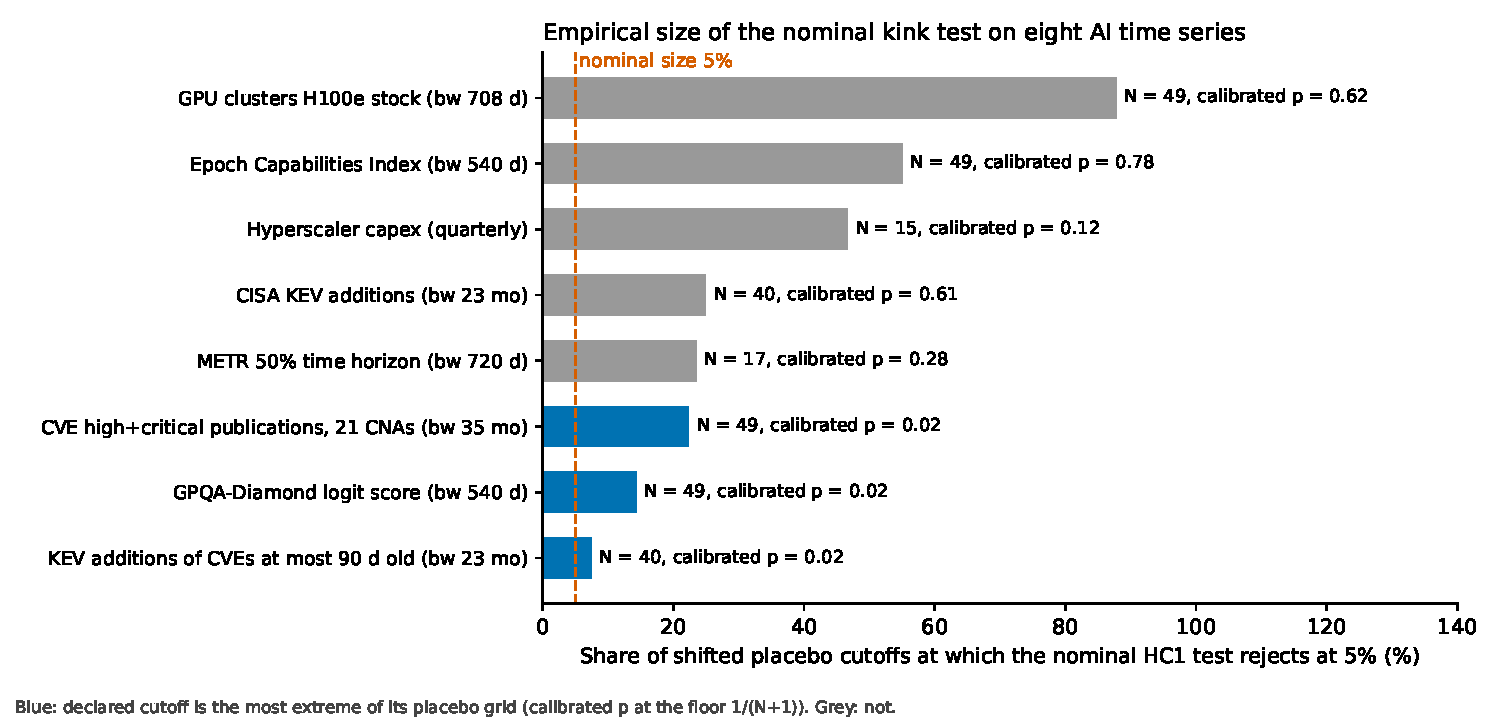
\includegraphics[width=\textwidth]{placebo_size}
\caption{Empirical size of the nominal kink test at shifted placebo cutoffs. Blue bars
mark series whose declared cutoff is the most extreme of its grid. Data:
\code{figures/placebo\_size.csv}.}
\label{fig:size}
\end{figure}

\begin{table}[t]
\centering
\small
\caption{Placebo grids on eight AI time series. $N$ is the number of evaluable placebo
cutoffs; the rejection rate is the share at which the nominal HC1 test rejects at 5\%.}
\label{tab:size}
\begin{tabular}{@{}p{5.6cm}lrrrl@{}}
\toprule
Series & Event & $N$ & Rejection & $p_{\mathrm{cal}}$ & Verdict \\
\midrule
GPQA-Diamond logit score & o1-preview & 49 & 14\% & 0.020 & dated bend \\
METR 50\% time horizon & o1-preview & 17 & 24\% & 0.278 & era bend \\
Epoch Capabilities Index & o1-preview & 49 & 55\% & 0.780 & null \\
GPU clusters, H100e stock & ChatGPT & 49 & 88\% & 0.620 & null \\
Hyperscaler capex, quarterly & ChatGPT & 15 & 47\% & 0.125 & inconclusive \\
CVE high and critical, 21 CNAs & Mythos & 49 & 22\% & 0.020 & dated bend \\
CISA KEV additions & April 2026 & 40 & 25\% & 0.610 & null \\
KEV additions of CVEs at most 90 days old & April 2026 & 40 & 8\% & 0.024 & dated bend \\
\bottomrule
\end{tabular}
\end{table}

\subsection{Worked example: vulnerability disclosure and exploitation after Claude Mythos}\label{sec:worked}

Anthropic announced Claude Mythos and Project Glasswing on 7 April 2026, with eight
founding partners that included several large vendors and the Linux Foundation. The
question was whether vulnerability disclosure bent at that date and whether exploitation
followed. The data are the CVE Program's cvelistV5 bundle of 2 October 2026 \cite{cvelist} and the
CISA Known Exploited Vulnerabilities catalogue of the same day \cite{kev}. The CVE records
are aggregated to an organisation by month panel over Epoch AI's 21 notable CVE numbering
authorities.

Table~\ref{tab:cve} reports the kink at April 2026 in the log of monthly high and
critical publications, with its robustness and placebo-date rows. The pooled slope
change is 3.9 log points per year. It is the most extreme of 49 placebo dates. It holds when the Linux kernel authority, the
founding partners, or the non-partners are removed in turn. Shifting the declared date to April 2025 or April 2024 gives calibrated
$p$-values of 0.18 and 0.86. Blind SuDDDS scans, told nothing about the date, put the
jump at April or May 2026 for all 21 authorities. A two-way fixed-effects contrast of founding partners against the other 13 authorities
after April 2026 is 0.42 log points. Its cluster-robust $p$ is 0.33 and its placebo-in-
space $p$ is 0.41 over 1{,}999 reassignments. The surge is broad-based; these data do not attribute it to the partners.

\begin{table}[t]
\centering
\small
\caption{Kink at April 2026 in log monthly high and critical CVE publications, 35-month
bandwidth. Slope changes are in log points per year.}
\label{tab:cve}
\begin{tabular}{@{}lrrrrr@{}}
\toprule
Series & Slope change & $z$ & $N$ & Rejection & $p_{\mathrm{cal}}$ \\
\midrule
21 notable CNAs & 3.88 & 11.7 & 49 & 22\% & 0.02 \\
without the Linux kernel CNA & 3.96 & 11.7 & 49 & 41\% & 0.02 \\
13 non-partner CNAs & 5.12 & 7.7 & 49 & 45\% & 0.02 \\
8 founding partners & 3.23 & 9.1 & 49 & 51\% & 0.02 \\
all CNAs & 2.52 & 15.3 & 49 & 35\% & 0.02 \\
21 notable CNAs, placebo date April 2025 & 0.72 & 2.4 & 49 & 27\% & 0.18 \\
21 notable CNAs, placebo date April 2024 & $-0.16$ & $-0.7$ & 49 & 51\% & 0.86 \\
\bottomrule
\end{tabular}
\end{table}

Exploitation did not keep pace (Table~\ref{tab:kev}). Total monthly additions to the KEV catalogue show no bend at April 2026. Blind scans put
the catalogue's sharpest change in 2022, when it was being populated. Additions of CVEs published within the previous 90
days did bend, by 1.7 log points per year, at the floor of a 40-position grid. Because
disclosures rose faster, the share of published CVEs that entered the catalogue within 30
days fell from 2.7 to 1.9 per thousand. The median lag from publication to catalogue entry fell from 7 to 4 days. The Mann--
Whitney $p$ is 0.12 on 189 and 149 entries, and the post-period lags are right-censored. A
vendor-level contrast of the seven partner vendors against 29 others after April 2026 is
0.14 log points. Its cluster-robust $p$ is 0.42 and its placebo-in-space $p$ is 0.19.

\begin{table}[t]
\centering
\small
\caption{Kinks at April 2026 in log monthly KEV additions, 23-month bandwidth.}
\label{tab:kev}
\begin{tabular}{@{}lrrrrr@{}}
\toprule
Series & Slope change & $z$ & $N$ & Rejection & $p_{\mathrm{cal}}$ \\
\midrule
all additions & 0.81 & 1.1 & 40 & 25\% & 0.61 \\
additions of CVEs at most 90 days old & 1.74 & 3.8 & 40 & 8\% & 0.02 \\
additions within 30 days of publication & 1.18 & 1.8 & 40 & 3\% & 0.12 \\
\bottomrule
\end{tabular}
\end{table}

\subsection{An honest miss}\label{sec:miss}

One collection note documents a failure of the level-break scan on a diffusion process
\cite{chinchillanote}. A blind LoRD3 scan of $\log_{10}$ training tokens per parameter over calendar time was run
on 549 language models. It returned a single significant discovery centred on 22 September
2022. The known event, the Chinchilla scaling result of 29 March
2022, ranks 158th of 547 candidates. The discovered break is six months late and points the wrong way. Fine-tuned releases
enter the panel with token counts that cover only the fine-tuning run. Two rules follow. Diffusion-style treatments need a slope
statistic, not only a level-break statistic. And fine-tune rows must be filtered from
tokens-per-parameter panels before any scan.

\section{Discussion and limitations}\label{sec:limits}

What the calibrated $p$ establishes is narrow. It says that the declared date is more
extreme than every shifted date on the same series under the same estimator. It does not
say what caused the bend. For the CVE series, the April 2026 bend coincides with the Mythos announcement. These data
cannot attribute it to Mythos, to Glasswing, or to any single cause. The partner contrast
is null and the bend is present in every authority group. For the GPQA-Diamond series the bend coincides with the entry of
reasoning models into the release stream, and composition is the mechanism. A dated bend
is a dated bend.

The limitations are these. Calendar-time kinks rest on one untestable assumption: no other slope-changing event is
co-located with the declared date. Placebo calibration tests exchangeability of dates, not
that assumption. HAC covariances are a mitigation on
short persistent windows, not a certificate, which is why they do not decide verdicts.
Robust bias correction for the local-polynomial fits is not implemented, so bandwidth
and polynomial sensitivity are part of every analysis. The did family estimates effects
for the configuration's single declared outcome; per-outcome effects exist only for rdd.
The sc family can pick a time-invariant group indicator as the treatment on some panels,
which is an open issue. The plug-in Lasso assumes a noisy first stage and over-selects
when assignment is a deterministic step function. Synthetic controls fit outcomes only,
without covariate weights. The analyst backends order the scan and never touch a statistic. A language model can
neither improve nor corrupt the numbers. It can only change which configuration is
reported first. The sixteen companion notes written under 0.2.0 have not been re-run under these rules. A
calendar-time result in them that rests on a seven-placebo grid has a floor of 0.125. It
is not a 5\% finding.

\section{Reproducibility}\label{sec:repro}

\natex{} is a Python package with core dependencies limited to numpy, scipy, pandas,
scikit-learn, typer and pydantic. Every stochastic call takes one
\code{numpy.random.Generator}; a run replays bitwise from its seed. The offline test suite collects 1{,}269 tests and runs on Python 3.11 to 3.14 in
continuous integration. The 32 real-data backtests of Section~\ref{sec:backtests} run
against a local data directory that is never committed. The first four series of
Section~\ref{sec:field} are taken from the flagship paper's case-study file. The fifth is
from the capex note. The last three are from the archived October 2026 runs. The figure is drawn from the
committed file \code{figures/placebo\_size.csv} by \code{make\_figures.py}. Source,
method cards, the reconciled audit and the release notes for 0.3.0 are in the
repository \cite{natex}.

\appendix

\section{Placebo grid construction}\label{app:grid}

Given a running variable $r$, a declared cutoff $c$, a bandwidth $h$ and a target of
$N^\ast = 49$ positions:
\begin{enumerate}
\item Take the distinct values of $r$ between its 10th and 90th percentiles.
\item Drop values with $|r - c| \le h/4$.
\item If more than $N^\ast$ remain, keep $N^\ast$ evenly spaced in rank order.
\item At each remaining value re-estimate the kink with the headline bandwidth, kernel,
degree, donut and covariance. Positions where a cell lacks residual degrees of freedom
are dropped. $N$ counts the evaluable remainder.
\item Report $p_{\mathrm{cal}}$, $N$ and the floor $1/(N+1)$. Report the share of
positions with nominal $p \le 0.05$.
\end{enumerate}
The minimum of 19 positions is the smallest $N$ for which the floor is at most 0.05.

\begin{thebibliography}{99}

\bibitem{abadie2010}
Abadie, A., Diamond, A., and Hainmueller, J. (2010).
Synthetic control methods for comparative case studies: Estimating the effect of
California's tobacco control program.
\emph{Journal of the American Statistical Association}, 105(490), 493--505.

\bibitem{anderson1949}
Anderson, T.~W., and Rubin, H. (1949).
Estimation of the parameters of a single equation in a complete system of stochastic
equations.
\emph{Annals of Mathematical Statistics}, 20(1), 46--63.

\bibitem{belloni2012}
Belloni, A., Chen, D., Chernozhukov, V., and Hansen, C. (2012).
Sparse models and methods for optimal instruments with an application to eminent domain.
\emph{Econometrica}, 80(6), 2369--2429.

\bibitem{bockerman2025}
B\"ockerman, P., Jysm\"a, S., and Kanninen, O. (2025).
\emph{Difference-in-Kinks Design}.
IZA Discussion Paper No.~18313.
\url{https://docs.iza.org/dp18313.pdf}

\bibitem{card2015}
Card, D., Lee, D.~S., Pei, Z., and Weber, A. (2015).
Inference on causal effects in a generalized regression kink design.
\emph{Econometrica}, 83(6), 2453--2483.

\bibitem{capexnote}
Hillebrandt, H. (2026).
A genuine bend, no causal certificate: hyperscaler capex at ChatGPT.
\natex{} paper collection, companion note.
\url{https://haukehillebrandt.github.io/natex/capex-dik-chatgpt/}

\bibitem{chinchillanote}
Hillebrandt, H. (2026).
An honest miss: Chinchilla as an adoption ramp.
\natex{} paper collection, companion note.
\url{https://haukehillebrandt.github.io/natex/chinchilla-writeup/}

\bibitem{flagship}
Hillebrandt, H. (2026).
Placebo-calibrated kink tests of four claimed trend breaks in Epoch AI data.
\natex{} paper collection, flagship paper.
\url{https://haukehillebrandt.github.io/natex/paper/}

\bibitem{prop99note}
Hillebrandt, H. (2026).
Recovering Proposition 99 blind: validating the \natex{} pipeline against the
Abadie--Diamond--Hainmueller benchmark.
\natex{} paper collection, companion note.
\url{https://haukehillebrandt.github.io/natex/prop99-validation-writeup/}

\bibitem{natex}
Hillebrandt, H. (2026).
\emph{natex: automated natural-experiment discovery and estimation} (version 0.3.0).
Software.
\url{https://github.com/HaukeHillebrandt/natex}

\bibitem{cvelist}
CVE Program (2026).
cvelistV5, release \texttt{cve\_2026-10-02\_1400Z}.
\url{https://github.com/CVEProject/cvelistV5}

\bibitem{kev}
Cybersecurity and Infrastructure Security Agency (2026).
Known Exploited Vulnerabilities Catalog, 2 October 2026.
\url{https://www.cisa.gov/known-exploited-vulnerabilities-catalog}

\bibitem{fieller1954}
Fieller, E.~C. (1954).
Some problems in interval estimation.
\emph{Journal of the Royal Statistical Society, Series B}, 16(2), 175--185.

\bibitem{herlands2018}
Herlands, W., McFowland~III, E., Wilson, A.~G., and Neill, D.~B. (2018).
Automated local regression discontinuity design discovery.
In \emph{Proceedings of the 24th ACM SIGKDD International Conference on Knowledge
Discovery and Data Mining (KDD~'18)}.

\bibitem{herlands2020}
Herlands, W. (2020).
\emph{Change Modeling for Understanding Our World and the Counterfactual One(s)}.
PhD thesis, Carnegie Mellon University.

\bibitem{holm1979}
Holm, S. (1979).
A simple sequentially rejective multiple test procedure.
\emph{Scandinavian Journal of Statistics}, 6(2), 65--70.

\bibitem{jakubowski2023}
Jakubowski, B., Somanchi, S., McFowland~III, E., and Neill, D.~B. (2023).
Exploiting discovered regression discontinuities to debias conditioned-on-observable
estimators.
\emph{Journal of Machine Learning Research}, 24(133), 1--57.

\bibitem{kleven2016}
Kleven, H.~J. (2016).
Bunching.
\emph{Annual Review of Economics}, 8, 435--464.

\bibitem{mccrary2008}
McCrary, J. (2008).
Manipulation of the running variable in the regression discontinuity design: A density
test.
\emph{Journal of Econometrics}, 142(2), 698--714.

\end{thebibliography}

\end{document}
